The muon system \cite{MuonTDR} is responsible for recording the momenta of muons in the outer-most layer of CMS. As muons provide a clean signature in many physics analyses, obtaining high-resolution measurements of muon momenta is critical. It is comprised of four separate technologies that provide redundancy in both the barrel and endcap regions. The subsystems are the Drift Tubes (DTs) in the barrel, the Cathode Strip Chambers (CSCs) and in the endcap regions, the Resistive Plate Chambers (RPCs) in both the barrel and endcaps, and as of Run 3, the Gas Electon Multipliers (GEMs) located at the outer-most layer of the endcaps. Each subsytem uses a different technology and records muon hits separetly, with reconstruction combining the information from all the subsytems. The muon barrel (MB) system is divided into four concentric shells, or stations, in each of the five wheels of the CMS barrel, labeled from inner-most to outer-most (along the $r$-coordinate): MB1, MB2, MB3, and MB4. Similarly, the muon endcap (ME) system is arranged into four disks in both the plus and minus endcaps, also called stations, labeled from inner-most to outer-most (along the $z$-coordinate): ME$\pm$1, ME$\pm$2, ME$\pm$3, and ME$\pm$4 ($\pm$ of course identifies the plus or minus endcap). Figure~\ref{fig:MuonSystem} shows a diagram including each subsytem and the pseudorapidity coverage of the muon system.

\begin{figure}[H]
    \centering
    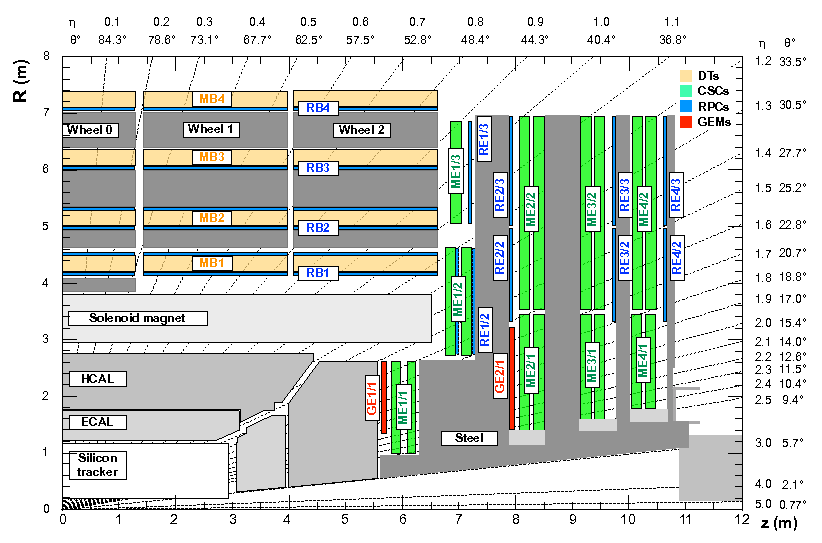
\includegraphics[width=1\textwidth]{Images/CMS/MuonSystem.png}
    \caption{A cutaway schematic of one quadrant of the muon system. Included are the CSCs, DT chambers, RPCs, and GEM detectors.}
    \label{fig:MuonSystem}
\end{figure}

\subsubsection{Cathode Strip Chambers} \label{sec:CSC}
% Introduce detector, location, basic info (e.g., chamber count)
% What is the technology
% Anatomy of a chamber
% How are they arranged in the barrel/endcap
% What do they measure
% Coverage
% Performance

Providing coverage in the plus and minus MEs within $0.9<|\eta|<2.4$ are the Cathode Strip Chambers (CSCs), which occupy the four ME stations along with RPCs. CSCs are labeled by ME station $\pm$n, then by ring m, like ``ME$\pm$n/m.'' In ME$\pm$2 to ME$\pm$4, each station consists of two concentric rings of CSCs, while ME$\pm$1 supports three rings of chambers (see Fig.~\ref{fig:CSC}). All rings contain 36 chambers, except for the outer-most rings of stations 2-4 (ME$\pm$2/2, ME$\pm$3/2, and ME$\pm$4/2) which hold only 18 chambers, for a total of 540 CSCs. Within each ring, CSCs are azimuthally overlapping with no gaps, offering full $\phi$ coverage. Each chamber is constructed from seven layers of polycarbonate honeycomb panels, with a gas mixture of 50\% Ar, 40\% CO2, and 10\% CF4 filling the six gaps between the panels. Embedded in a thin FR4 (fire-resistant fiberglass epoxy) surface on each panel are radially-extended cathode strips. Within each gap are azimuthally-running anode wires supplied with \SIrange{2.9}{3.5}{kV} of voltage. Muons passing through a chamber will locally ionize the gas in each gap, while the high voltage will induce a charge avalanche that drifts toward the cathode strips and an image charge will drift toward the anode wires (see Fig.~\ref{fig:CSCDiagram}). Each chamber provides a spacial resolution of \SIrange{50}{140}{\micro\meter} (depending on the chamber) and a timing resolution of \SI{3}{ns}.

\begin{figure}[H]
    \centering
    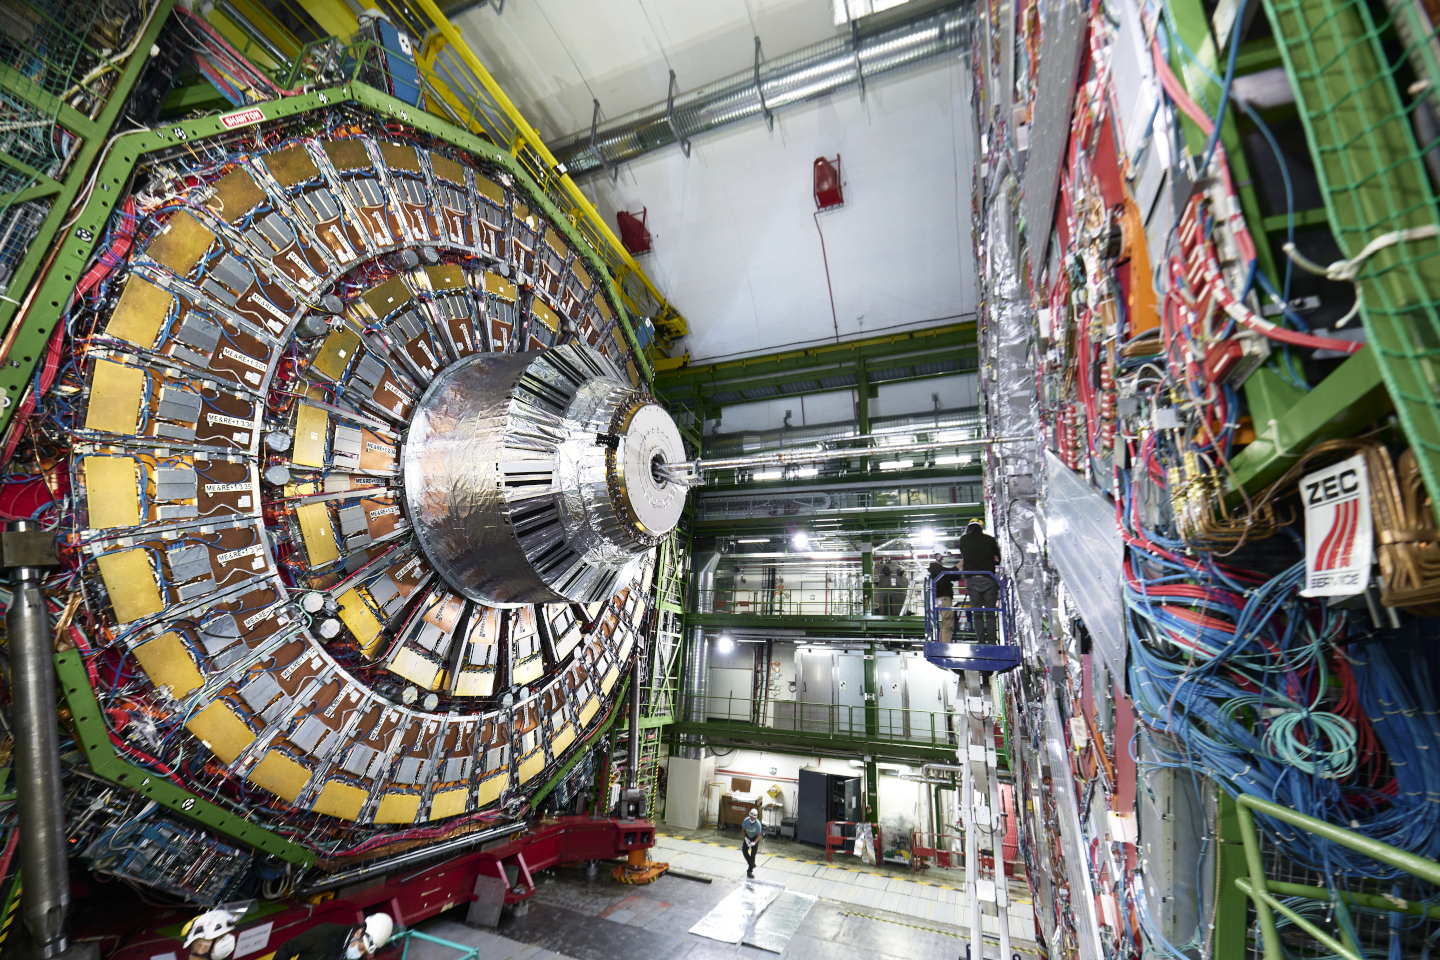
\includegraphics[width=1\textwidth]{Images/CMS/CSC.jpg}
    \caption{A photograph of CSCs mounted to the first endcap station.}
    \label{fig:CSC}
\end{figure}

\begin{figure}[H]
    \centering
    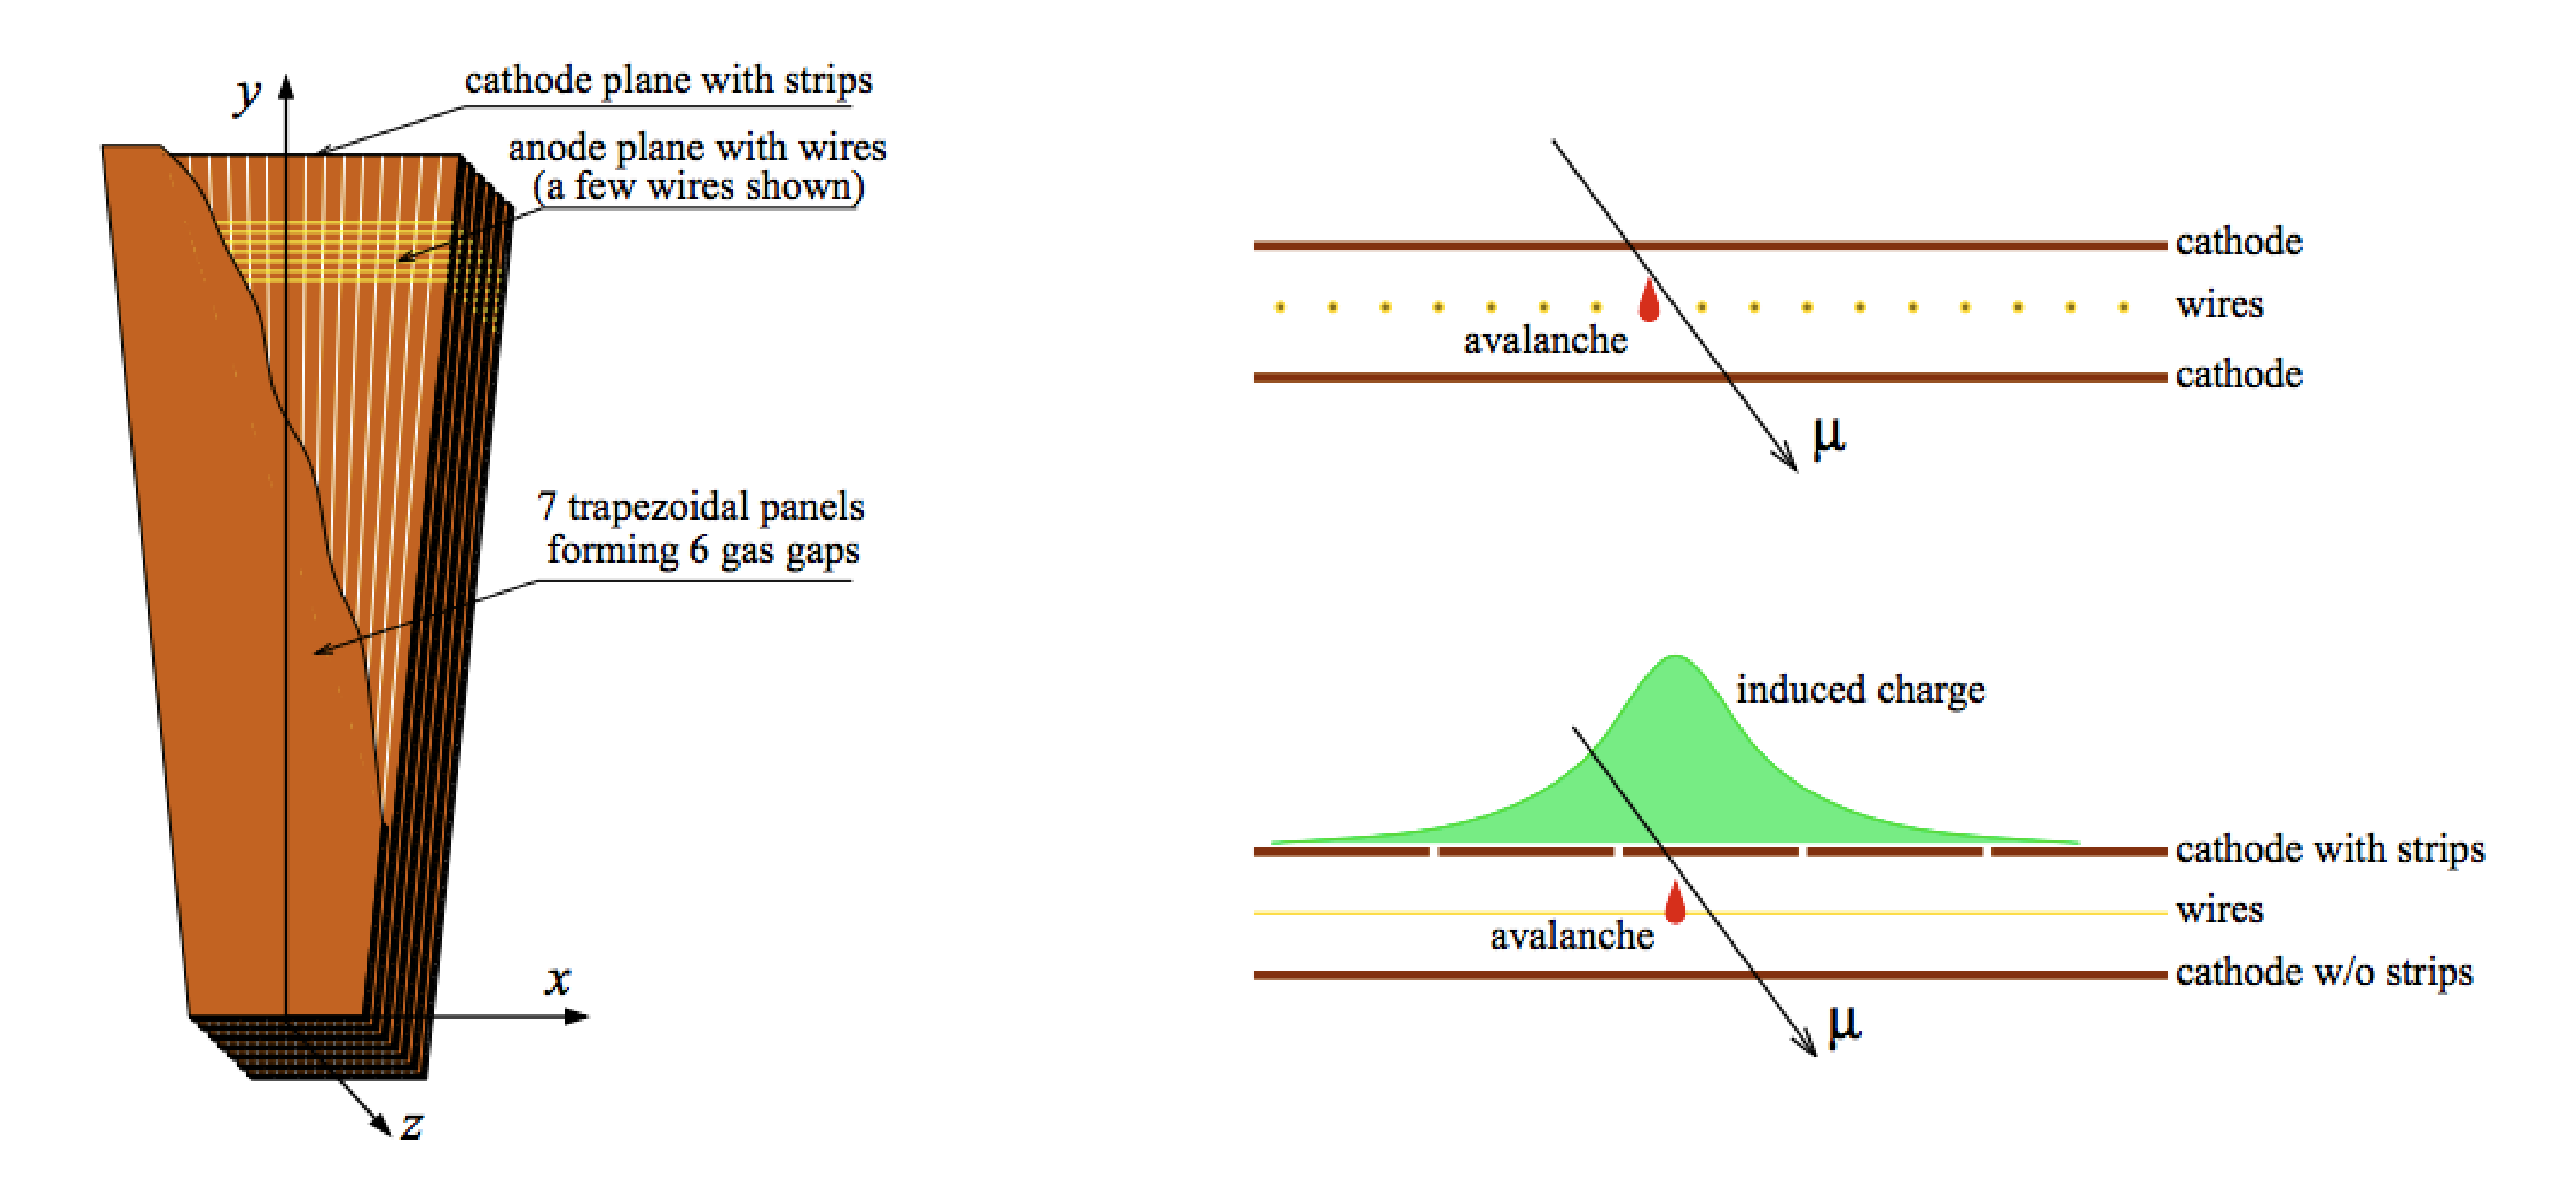
\includegraphics[width=\textwidth]{Images/CMS/CSCDiagram.png}
    \caption{Left: A schematic of a CSC. Right: A muon passing through a CSC will induce a charge avalanche.}
    \label{fig:CSCDiagram}
\end{figure}

\subsubsection{Drift Tubes} \label{sec:DT}

% Introduce detector, location, basic info (e.g., chamber count)
% What is the technology
% Anatomy of a chamber
% How are they arranged in the barrel/endcap
% Coverage
% What do they measure
% Precision
% Performance

Located in the MB are 250 Drift Tube (DT) chambers, layered between RPCs, and arranged to provide coverage within $|\eta|<1.2$ overlapping with the CSC coverage in the muon endcaps (see Fig.~\ref{fig:DT}). DT chambers are labeled by MB station n, then by wheel w, like ``MBn$\pm$w.'' A single DT consists of a long aluminum drift cell filled with a gas mixture of 85~\% Ar and 15~\% CO2 and a central anode wire strung length-wise inside the cell held at \SI{+3600}{V}. Electrode strips held at \SI{+1800}{V} and cathode strips held at \SI{-1200}{V} line the walls of each cell and help shape the electric field inside (see the diagram in Fig.~\ref{fig:DTDiagram}). In MB1-MB3, the DT chambers are grouped into three collections of four consecutive, stagered layers of drift tubes called Super Layers (SLs), while in MB4 there are only two SLs per chamber. The inner-most and outer-most SL in a DT chamber measure $r$-$\phi$ coordinates in the bending plane, while the middle SL measures along the $z$-coordinate. Between the outer-most and middle SL is a honeycomb layer that produces a $\SI{28}{cm}$ separation of measurements in the bending plane, which aid in determining muon track bending. In MB4, DT chambers consist only of the two SLs measuring the $r$-$\phi$-coordinate, with no honeycomb spacer or $z$-coordinate SL. The spatial resolution per cell is at least \SI{250}{\micro\meter}, corresponding to a roughly \SI{100}{\micro\meter} resolution per chamber, while the time resolution per DT chamber is \SI{2}{ns}.

\begin{figure}[H]
    \centering
    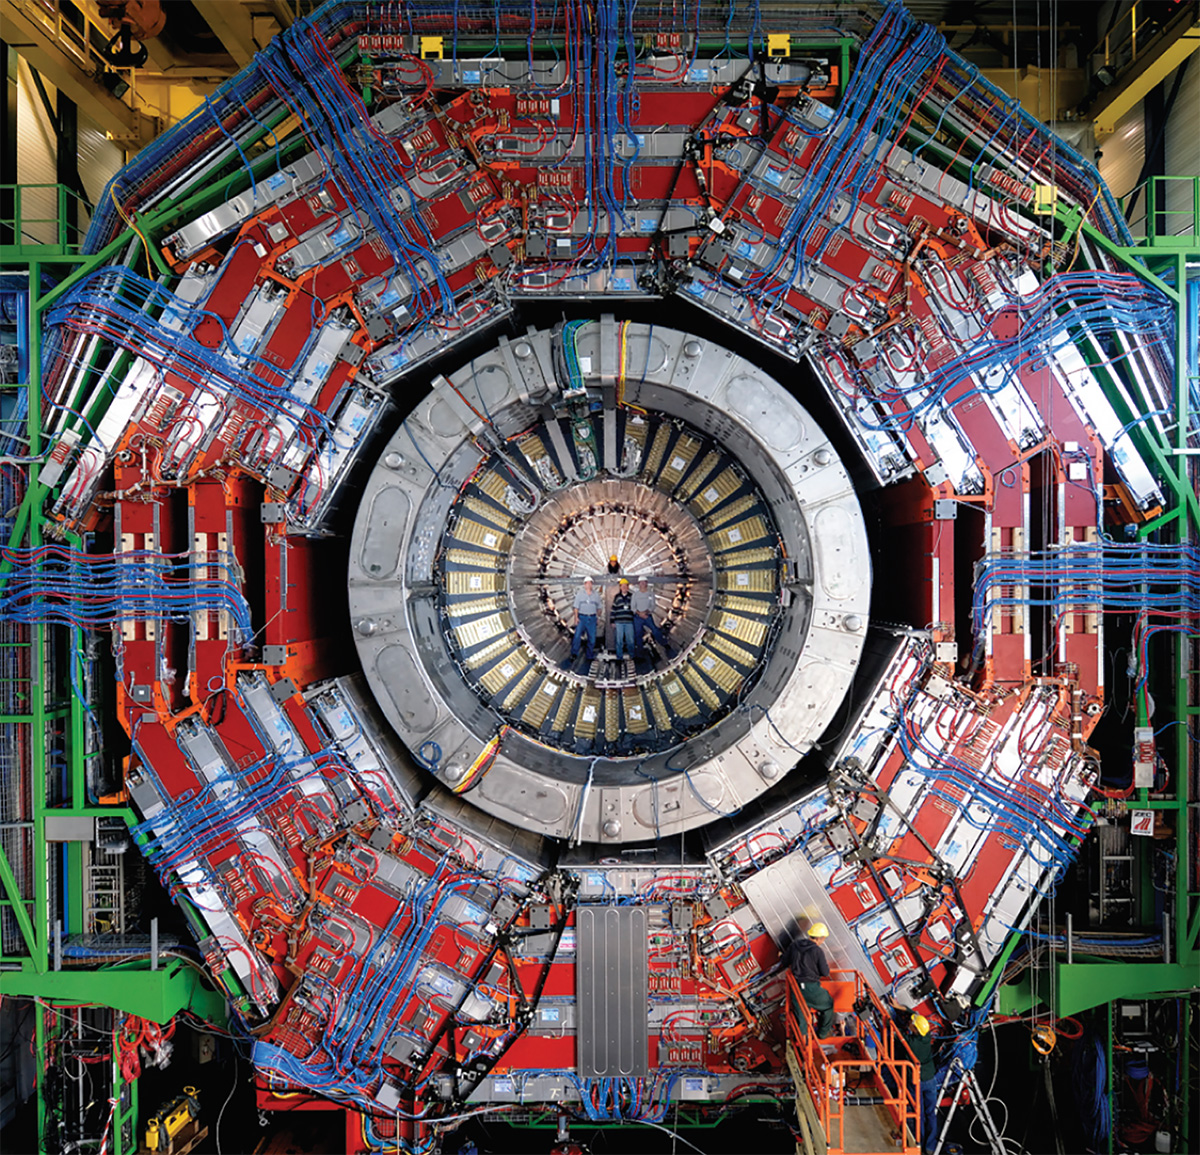
\includegraphics[width=\textwidth]{Images/CMS/DT.jpg}
    \caption{A photograph of DT chambers (silver boxes) installed in the return yoke (red structure) of a wheel in the muon barrel.}
    \label{fig:DT}
\end{figure}

\begin{figure}[H]
    \centering
    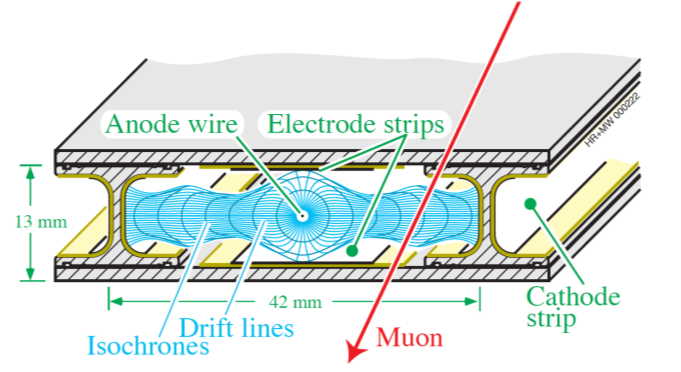
\includegraphics[width=1\textwidth]{Images/CMS/DTDiagram.png}
    \caption{A diagram of a single DT chamber.}
    \label{fig:DTDiagram}
\end{figure}

\subsubsection{Resistive Plate Chambers} \label{sec:RPC}
% Introduce detector, location, basic info (e.g., chamber count)
% What is the technology
% Anatomy of a chamber
% How are they arranged in the barrel/endcap
% What do they measure
% Coverage
% Performance

Complementing the DT chambers and CSCs are the Resistive Plate Chambers (RPCs) located in both the MB and ME (shown in Fig.~\ref{fig:RPC}). RPCs have two naming conventions, depending on the region of the detector they occupy: in the barrel, ``RBn$\pm$w,'' and in the endcaps, ``RE$\pm$n/m,'' where ($\pm$)n denotes the MB or ME$\pm$ station (1-4), $\pm$w the MB wheel (1-5), and m the ME ring (1, 2, or 3 in RB$\pm$1; 1or 2 in all other stations). Pseudorapidity coverage by the RPCs overlaps with the other muon subsytems at $0.0 < |\eta| < 1.9$. In stations RB1 and RB2, two RPCs sandwich each DT chamber, while in RB3 and RB4, anywhere from one to four RPCs (depending on the station and sector) are layered on the inside of a single DT chamber. This leads to 480 total RPCs in the barrel. In the endcaps, RPCs are mounted to the opposite side of a yoke disk as the CSCs, forming alternating layers of CSCs and RPCs, and totalling 576 RPCs in the endcaps. Each RPC is a \SI{2}{mm} double-gap chamber, using Bakalite (a high pressure laminate) electrodes, operated in avalanche mode (see the diagram in Fig.~\ref{fig:RPCDiagram}). Electrode strips are longitudinally-running and segmented into two or three parts, depending on the station/sector. A RPC detector is optimized to record accurate timing and fast triggering, as well as identification the associated bunch crossing for a given muon track. Compared to the DTs and CSCs, RPCs have a coarse-grain spatial resolution of only 0.8 to \SI{1.3}{\cm}, but provide excellent timing resolution at \SI{1.5}{\ns}.

\begin{figure}[H]
    \centering
    {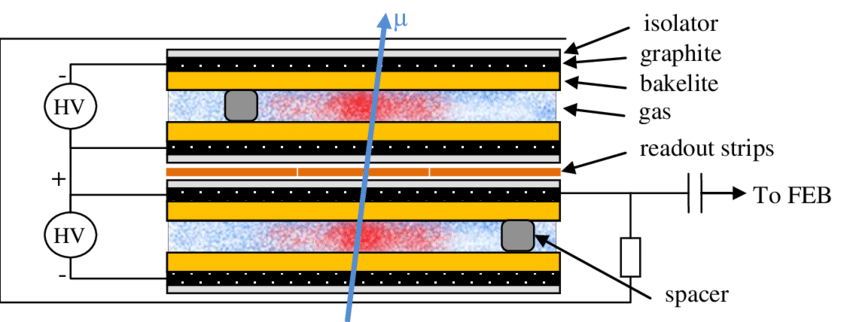
\includegraphics[width=\textwidth]{Images/CMS/RPCDiagram.png}}
    \caption{A diagram of an RPC.}
    \label{fig:RPCDiagram}
\end{figure}


\begin{figure}[H]
    \centering
    {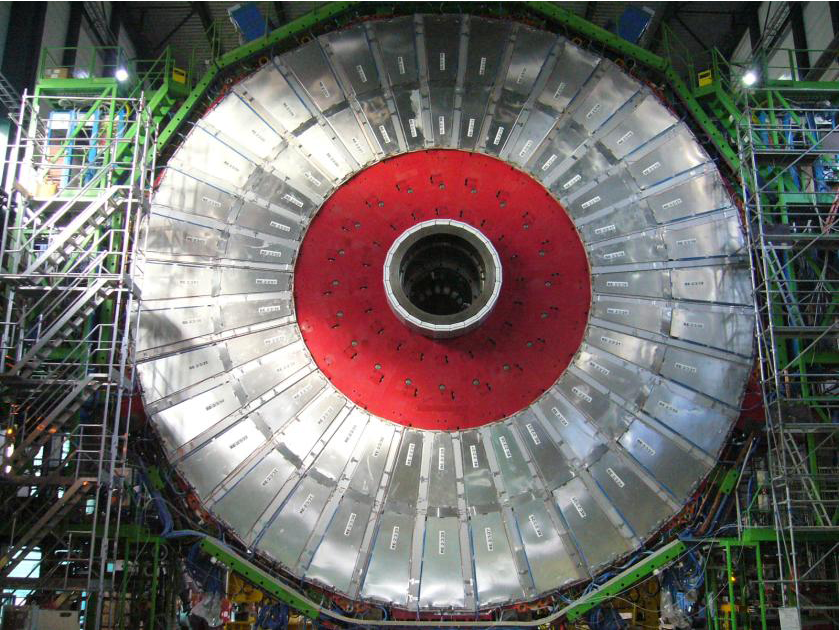
\includegraphics[width=1\textwidth]{Images/CMS/RE.png}}
    \caption{A photograph of RPCs mounted to the second endcap station.}
    \label{fig:RPC}
\end{figure}

\subsubsection{Gas Electron Multipliers} \label{sec:GEM}
During LS2, Gas Electron Multipliers (GEMs) \cite{GEM} were installed as part of the Phase 2 upgrades to the muon system. Located in the very forward regions of each ME and complimenting the CSCs, the GEMs cover the pseudorapidity range of $1.5<|\eta|<2.8$ and are labeled ME$\pm$0, GE$\pm$1/1 and GE$\pm$2/1. Each GEM detector consists of a tripple-layer of copper-cladded polyimide foil into which are etched \SI{70}{\micro \meter} holes spaced \SI{70}{\micro\meter} apart, in a hexagonal geometry, as can be seen in the diagrams in Figs.~\ref{fig:GEMDiagram} and~\ref{fig:GEMDiagram2} (left). A 70 \% Ar and 30 \% CO$_2$ gas mixture fills mm-sized gaps between the foil layers and a voltage is applied is steps ranging from \SI{-3200}{V} to ground (see Fig.~\ref{fig:GEMDiagram2}, right). The foil layers are sandwitched between a drift PCB and a readout PCB with 3072 radial strips. A total of 144 GEM chambers were installed during LS2 occupying the GE$\pm$1/1 station/ring, with the remaining chambers, ME$\pm$0 and GE$\pm$2/1 to be installed in LS3. 

\begin{figure}[H]
    \centering
    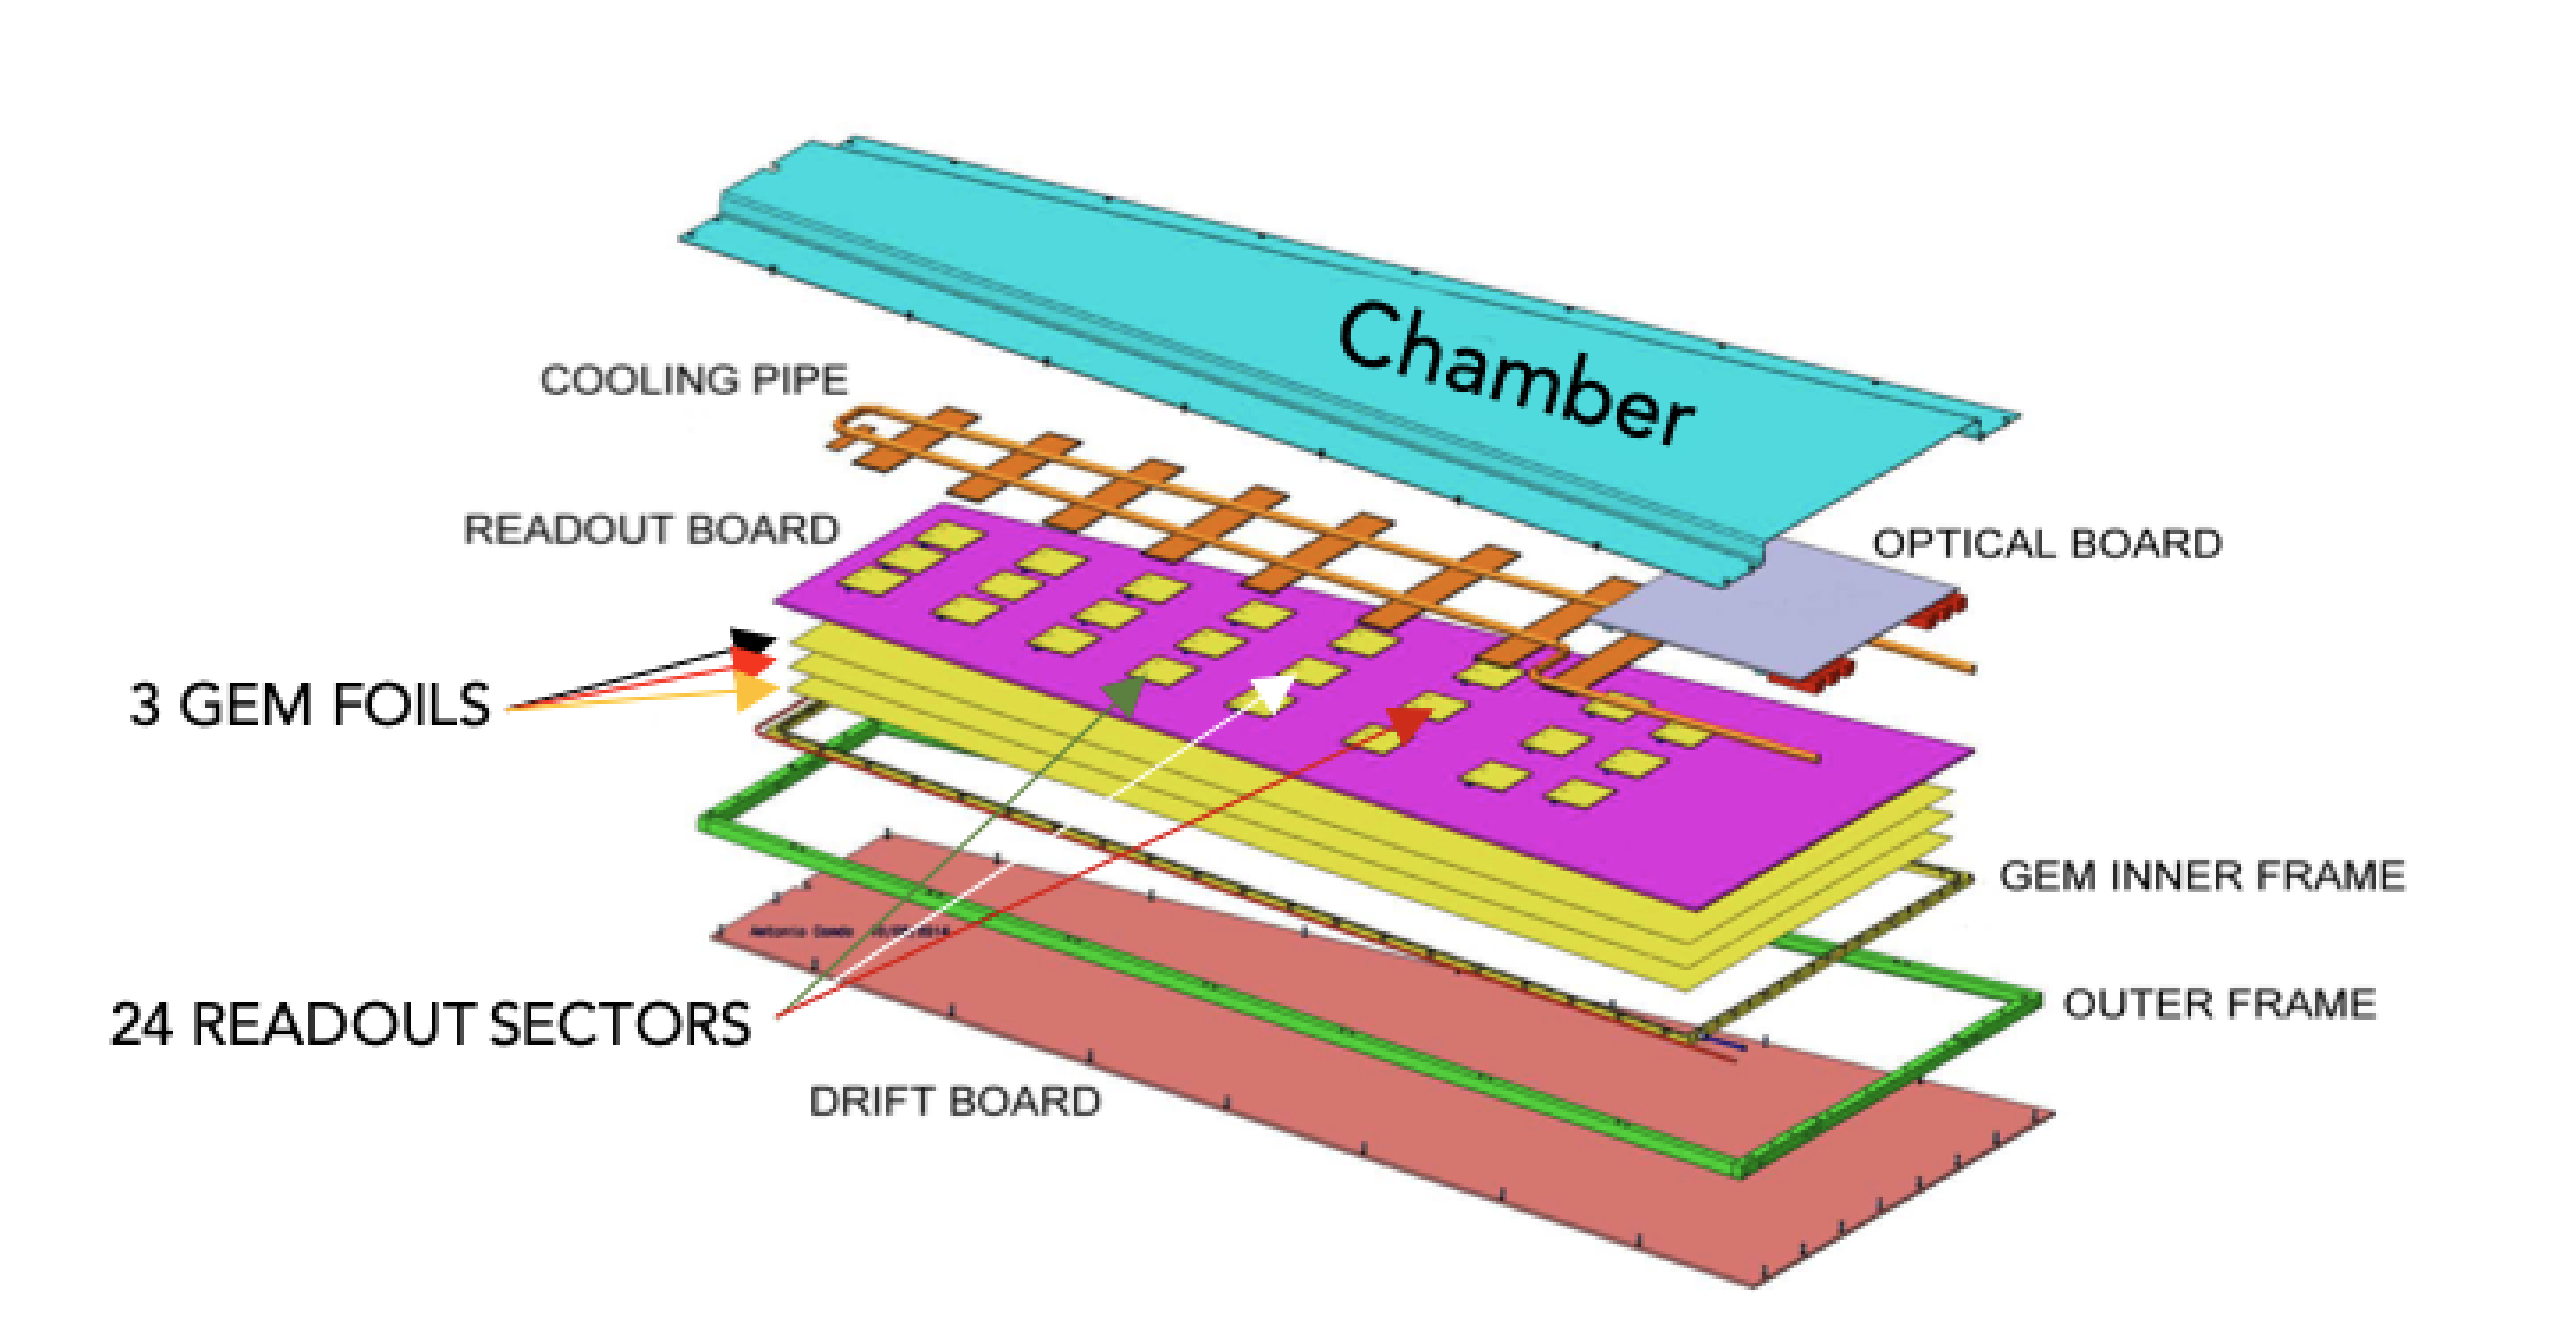
\includegraphics[width=\textwidth]{Images/CMS/GEMDiagram.png}
    \caption{An exploded view of a GEM chamber.}
    \label{fig:GEMDiagram}
\end{figure}

\begin{figure}[H]
    \centering
    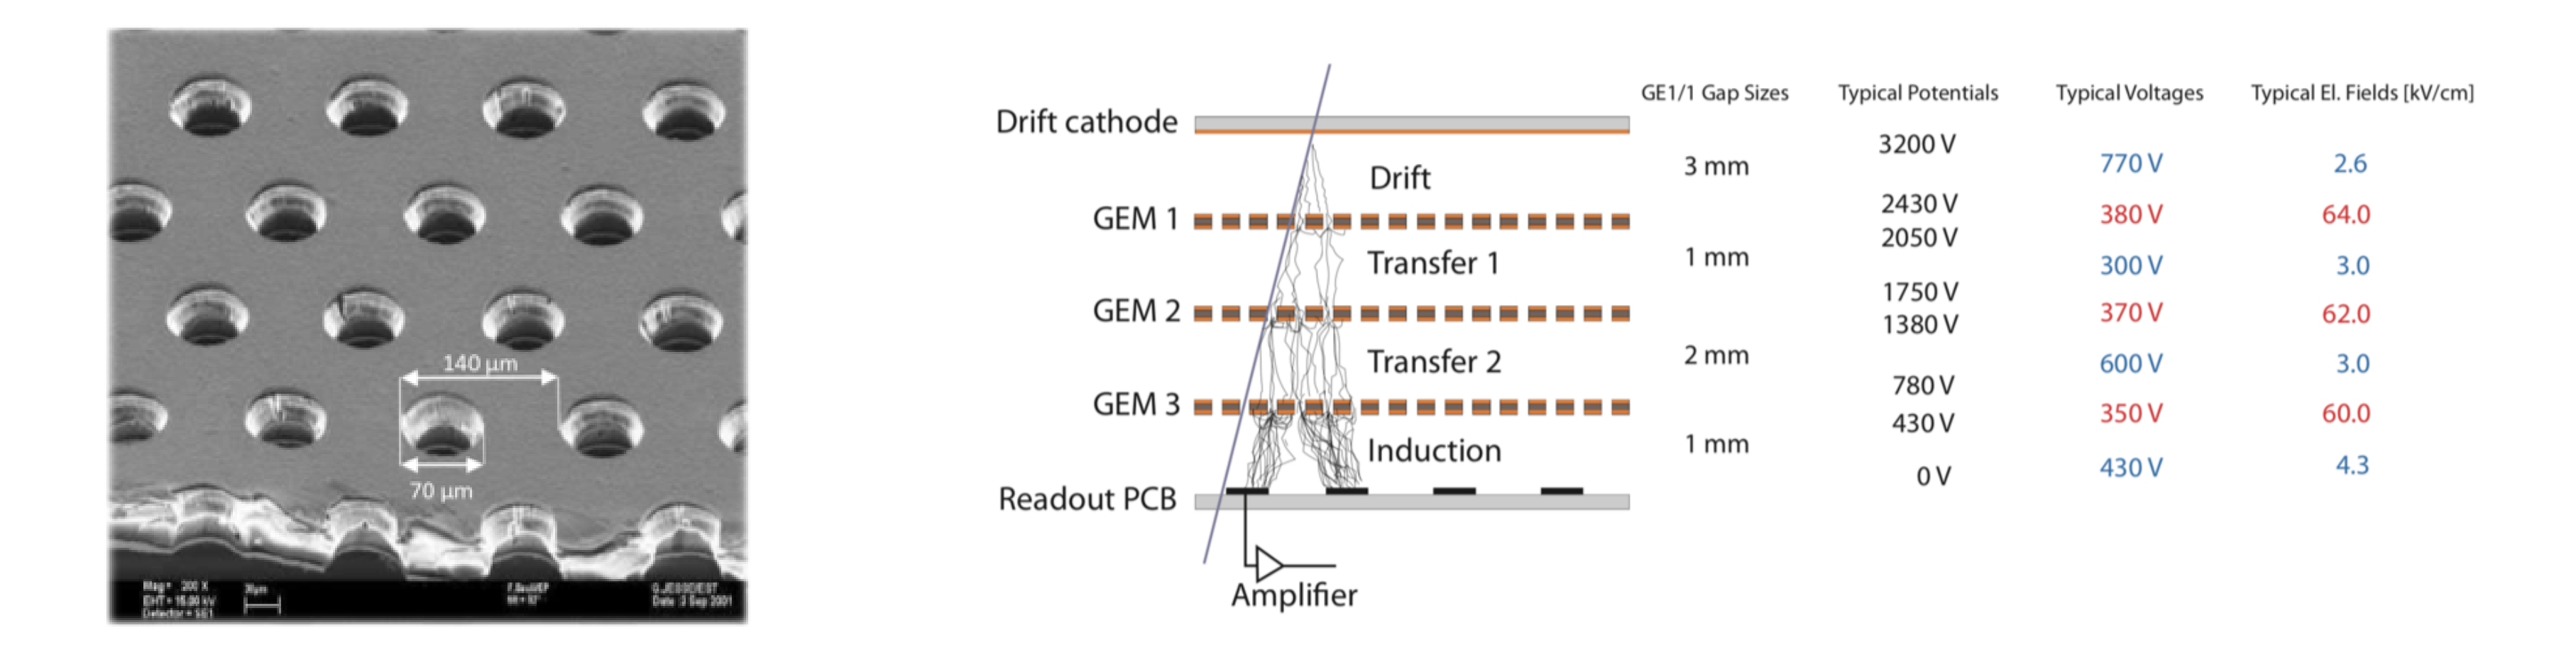
\includegraphics[width=\textwidth]{Images/CMS/GEMDiagram2.png}
    \caption{Left: a photograph of the micron-scale holes in the GEM foil. Right: The typical voltages in each layer of a GEM chamber.}
    \label{fig:GEMDiagram2}
\end{figure} 